\chapter{Decapole Measurements, Corrections and Modelling in the LHC}
\thumbforchapter{}
\chaptertoc{}
\newpage

% === Motivation
\section{Motivation}

The decapole fields in the LHC have been studied since Run 1 via chromaticity 
measurements~\cite{maclean_non-linear_2011,maclean_commissioning_2016,maclean_measurement_2014}. 
The third order of the non-linear chromaticity, $Q'''$, generated for the most part by decapoles,
has shown a consistent discrepancy at injection energy between its expected value in simulation and
that observed in beam-based measurements.
Figure \ref{fig:decapoles:bare_chroma_vs_simulations} highlights this discrepancy.

\begin{figure}[H]
    \centering
    %\captionsetup{justification=centering,margin=2cm}
    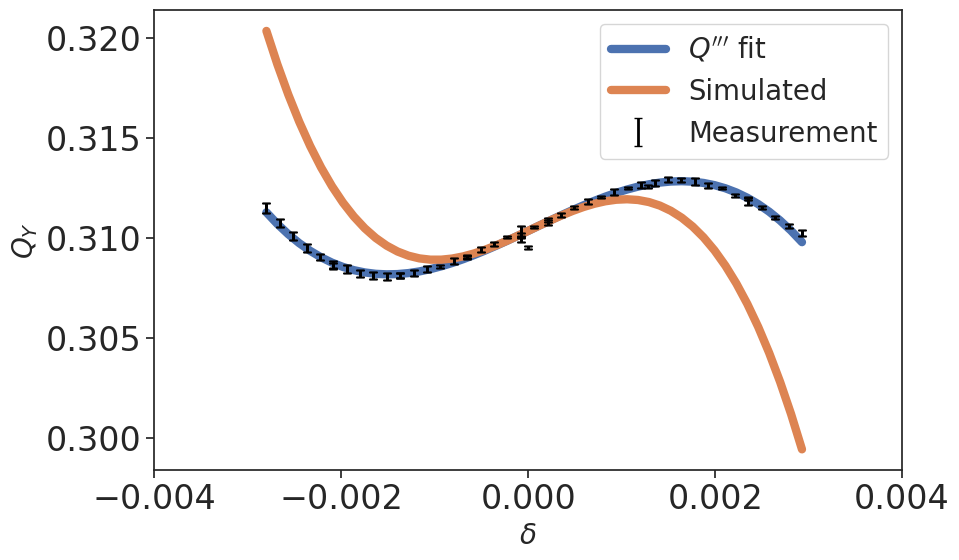
\includegraphics[width=0.7\textwidth]{images/bare_chroma_simulated.png}
    \caption{Measured and simulated chromaticity at injection energy without octupolar and
             decapolar corrections.}
    \label{fig:decapoles:bare_chroma_vs_simulations}
\end{figure}

This discrepancy poses a significant problem, as the operational corrections are derived from
simulations. It is thus observed that $Q'''$ is over-corrected by an almost factor 2, resulting in
an effectively un-corrected third order chromaticity.
Chromaticity measurements have thus been repeated during LHC's Run 3 and complemented by beam-based
corrections.

While non-linear chromaticity provides an easy measurement of decapolar fields, it does not permit
alone to understand where the discrepancy originates from. 
New measurements were therefore undertaken to better understand the decapolar fields via observables
never studied before:
\begin{itemize}
    \tightlist
    \item Bare Chromaticity, chromaticity with octupolar and decapolar correctors turned off.
    \item Chromatic Amplitude Detuning, tune shift dependant on both the action and the momentum 
    offset.
    \item Resonance Driving Term $f_{1004}$, contributing to a resonance close the working point.
\end{itemize}



% ===================
%    Chromaticity
% ===================


% Correction
%\paragraph{Correction}
%
%$Q'''$ is linear with the decapole strength. As such, it can be easily corrected via global trims
%presented in~\cref{subsection:correction_chromaticity}.
%A change of decapole strength $K_5 = 1000$ would for example have the following impact with the
%injection optics used in 2022:
%
%\begin{equation}
%    \begin{aligned}
%        \Delta Q'''_x =  1.5 \times 10^6 \quad;\quad
%        \Delta Q'''_y = -0.9 \times 10^6.
%    \end{aligned}
%\end{equation}






%\subsection{\todo{blabla}}
%
%Measurements were taken during 2022 Commissioning for 
%\begin{itemize}
%    \item Beam Test
%    \item Commissioning
%    \begin{itemize}
%        \item FiDeL
%        \item Q''' corr
%        \item Q'' corr
%    \end{itemize}
%    \item 60° optics
%\end{itemize}
%
%Also during MD6864, 2022-10-19, for the bare machine \\
%Also 2022-11-06, measurement at 30cm, flat top.
%

% ===============================
%        Corrector Response
% ===============================
\section{\review{Response of correctors}}

% ===============================
%         Introduction
\paragraph{Expression}

The full third term of the chromaticity function is highlighted in
\cref{eq:decapoles:chromaticity_highlight}. Details on chromaticity are given
in \cref{subsection:concepts:chromaticity}.

\begin{equation} 
    Q (\delta) = Q_0 + Q' \delta + \frac{1}{2!} Q'' \delta^2 
                     + \colorbox{yellow!50}{$\displaystyle  \frac{1}{3!}  Q''' \delta^3$}
                     + \mathcal{O}(\delta^4).
    \label{eq:decapoles:chromaticity_highlight}
\end{equation}

This third order, mainly contributed to by decapoles, is related to the $\beta$-function, the
dispersion and the strength of the multipole:

\begin{equation}
    \begin{aligned}
        \Delta Q_x''' &=  &\frac{1}{4\pi} K_{5} L \beta_x D_x^{3}\\
        \Delta Q_y''' &= -&\frac{1}{4\pi} K_{5} L \beta_x D_x^{3}.
    \end{aligned}
\end{equation}


% 2022-04-24
\paragraph{Measurements and Corrections}

In order to assess the accuracy of corrections, measurements have to be done to gauge the response
of the decapolar correctors, \textit{MCDs}.
During Run~3's commissioning, measurements and corrections of $Q''$ and $Q'''$ have been made
routine. Those corrections give the opportunity to study the response of the correctors.
\cref{figure:decapoles:chromaticity:dq3_comparison} shows the chromaticity function measured during
Run~3's commissioning in 2022 with the nominal corrections via FiDeL and beam-based corrections
computed analytically based on top of FiDeL.

\begin{figure}[H]
    \centering
    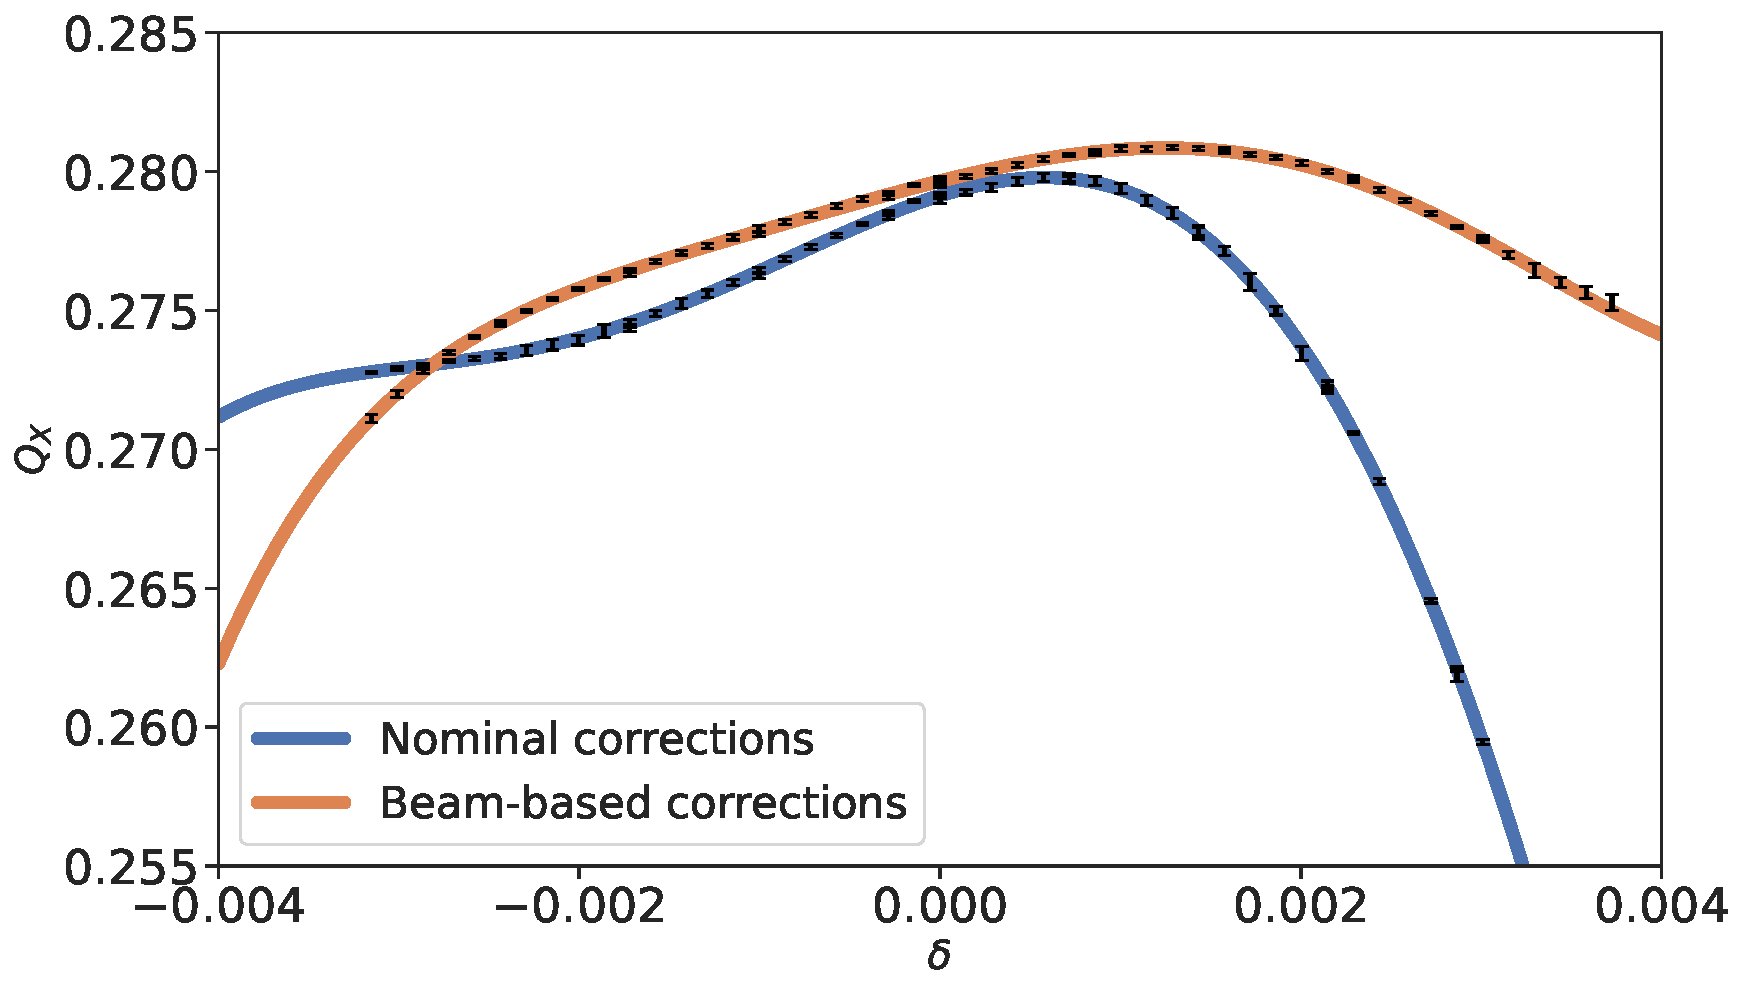
\includegraphics[width=0.8\columnwidth]{images/nominal_vs_beam_based_corrections.pdf}
    \caption{Chromaticity of the horizontal plane of Beam 1 during Run 3's commissioning, with
    nominal corrections based on the magnetic model and beam-based corrections aimed at correcting
     $Q''$ and $Q'''$.}
    \label{figure:decapoles:chromaticity:dq3_comparison}
\end{figure}

The nominal and corrected $Q'''$ values are shown in
\cref{table:decapoles:chromaticity:dq3_before_after_beam_based}. The shift in $Q'''$ is shown for
each beam and axis, showing a good agreement between the measurement and the simulation.
The slight imbalance can be attributed to higher order effects of the octupole correctors, whose
correction was implemented after that of $Q'''$.

\begin{table}[H]
    \centering
    \begin{tabular}{|l||r|r|r|c|}
    \hline
              &  \multicolumn{2}{c|}{$Q''' [10^6]$}  &  \multicolumn{2}{c|}{$\Delta Q''' [10^6]$}\\ \hline\hline
        B1    &   \multicolumn{1}{c|}{Nominal}     &   \multicolumn{1}{c|}{Beam-based}   & Measured & Simulated \\
        X     &  -3.36 ± 0.04 &  -1.02 ± 0.03  &  2.3 ± 0.1 &   2.5 \\
        Y     &   1.62 ± 0.05 &   0.12 ± 0.02  & -1.5 ± 0.1 &  -1.4 \\ \hline
        %B2    &   \multicolumn{1}{c|}{Nominal}     &   \multicolumn{1}{c|}{Beam-based}   &&\\
        B2    &               &&& \\
        X     &  -2.72 ± 0.08 &  -0.64 ± 0.03  &  2.1 ± 0.1 &  2.5\\
        Y     &   1.54 ± 0.06 &   0.14 ± 0.03  & -1.4 ± 0.1 & -1.4\\ \hline
    \end{tabular}
    \caption{Third order chromaticity obtained during Run~3 commissioning, with nominal and
    beam-based corrections aimed at correcting $Q''$ and $Q'''$.
    The change in $Q'''$, measured and expected via simulations, is also shown.} 
    \label{table:decapoles:chromaticity:dq3_before_after_beam_based}
\end{table}


This agreement between the simulations and the measurements indicates that our decapole correctors
function as intended. No noticeable cross-talk between magnets or hysteresis have been identified.



% ===============================
%        Bare Chromaticity
% ===============================
\section{\review{Bare Chromaticity}}


% 2022-10-19

Previous studies~\cite{maclean_measurement_2014} have demonstrated that octupole and decapole
correctors were contributing to an observed octupolar discrepancy in the machine via hysteresis and
feed-down. To evaluate the possible effect of decapole correctors on the third order chromaticity
$Q'''$, a measurement was taken with these elements turned off.

\begin{figure}[H]
    \begin{subfigure}{0.49\textwidth}
        \centering
        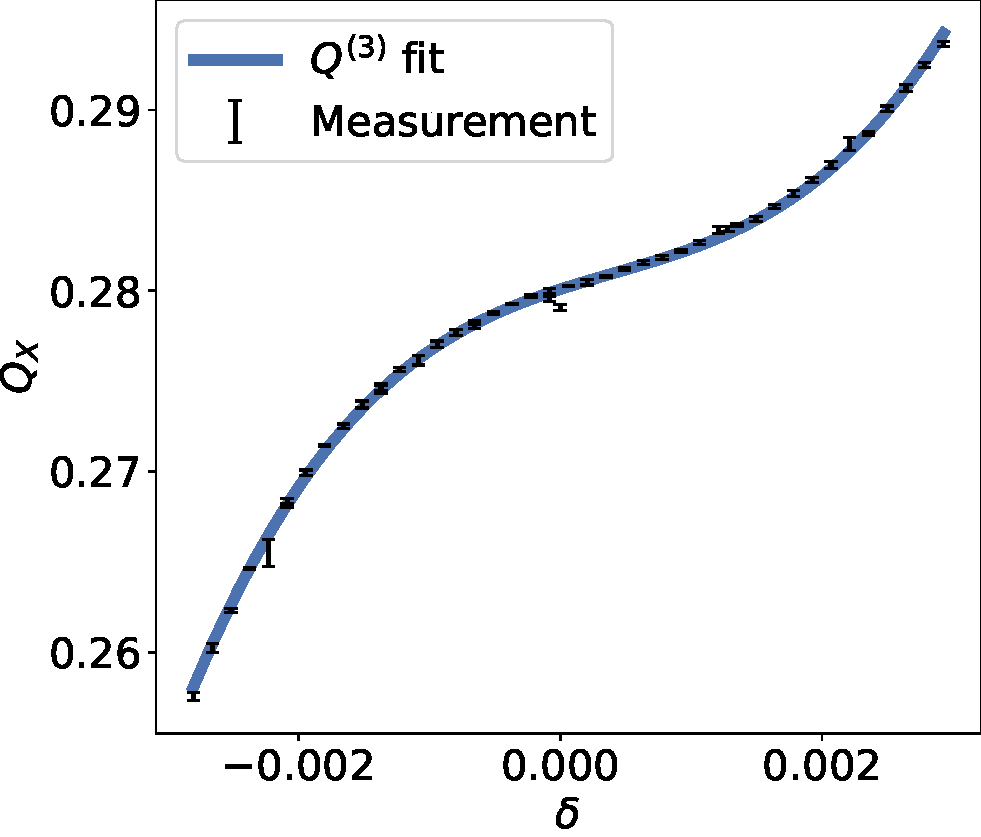
\includegraphics[width=\textwidth]{./images/bare_chromaticity/Beam1_Qx.pdf}
        \caption{$Q_x$ Beam 1}
        \label{}
    \end{subfigure}
    \hfill
    \begin{subfigure}{0.49\textwidth}
        \centering
        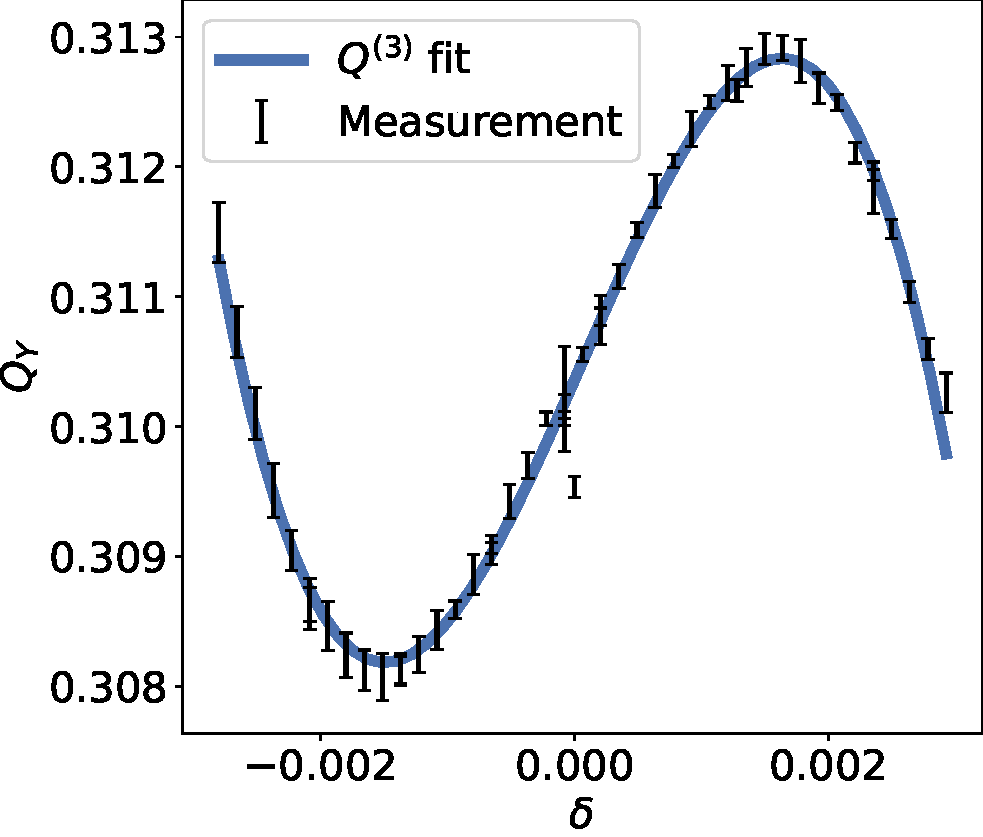
\includegraphics[width=\textwidth]{./images/bare_chromaticity/Beam1_Qy.pdf}
        \caption{$Q_y$ Beam 1}
        \label{}
    \end{subfigure}
    %
    \\
    %
    \begin{subfigure}{0.49\textwidth}
        \centering
        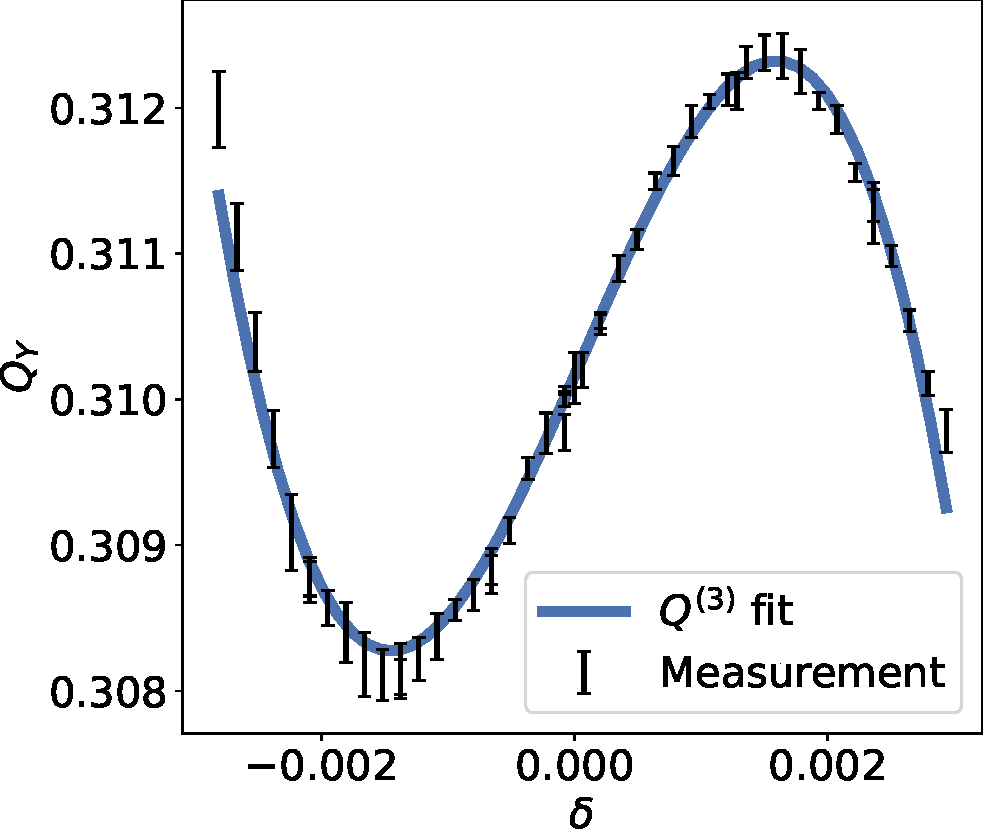
\includegraphics[width=\textwidth]{./images/bare_chromaticity/Beam2_Qy.pdf}
        \caption{$Q_x$ Beam 2}
        \label{}
    \end{subfigure}
    \hfill
    \begin{subfigure}{0.49\textwidth}
        \centering
        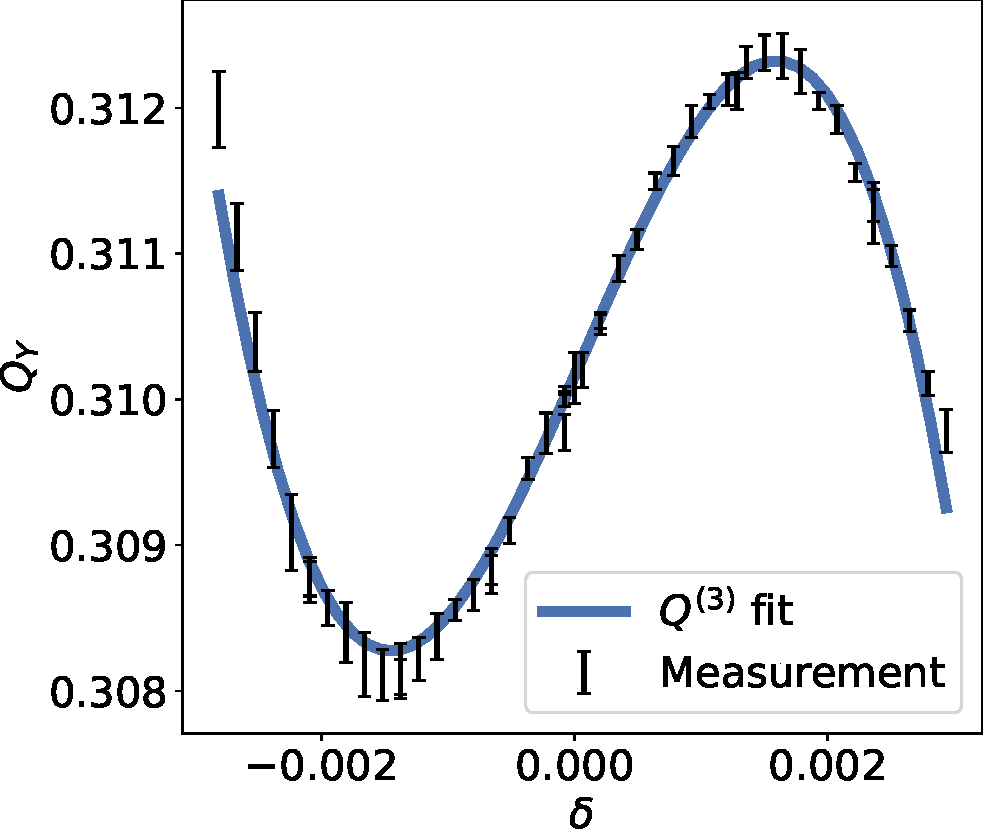
\includegraphics[width=\textwidth]{./images/bare_chromaticity/Beam2_Qy.pdf}
        \caption{$Q_y$ Beam 2}
        \label{}
    \end{subfigure}
    \caption{Fit of the chromaticity function for the chromaticity measurement performed with 
    octupole and decapole correctors powered off. The fit includes all orders up to third.}
    \label{fig:decapoles:bare_chromaticity}
\end{figure}

Simulations have been run with MAD-X and PTC including fields errors from $b_3$ to $b_8$. The
expected $Q'''$ values are presented in~\cref{table:decapoles:bare_chromaticity:virgin_dq3} and
compared to the measured ones along with the ratio between the two.

\begin{table}[tbh]
    \centering
    \begin{tabular}{|l||r|r|r|}
    \hline
        Plane     &  Meas. $Q''' [10^6]$        &  Sim. $Q''' [10^{6}]$          &   Ratio     \\\hline\hline
        Beam 1    &                             &                                &             \\
                X &            2.95 ± 0.04      &         6.94 ± 0.02            &  0.43 ± 0.01  \\
                Y &           -1.82 ± 0.04      &        -4.29 ± 0.01            &  0.42 ± 0.01  \\ \hline
        Beam 2    &                             &                                &             \\
                X &            3.06 ± 0.07      &        7.03 ± 0.02             &  0.44 ± 0.01 \\
                Y &           -1.72 ± 0.02      &       -4.27 ± 0.01             &  0.42 ± 0.01  \\ \hline
    \end{tabular}
    \caption{Measured and simulated third order chromaticity with octupole and decapole correctors
    turned off. The simulations include field errors from sextupoles to decahexapole ($b_3$ to
    $b_8$).}
    \label{table:decapoles:bare_chromaticity:virgin_dq3}
\end{table}

A consistent ratio is observed for every plane and axis between the measurement and the model. This
result, supplemented by the correct response of the correctors, indicates that the decapolar
correctors do no generate unwanted fields. Those correctors can thus be discarded as the potential
source of discrepancy.


% === Chromatic Amplitude Det
\section{Chromatic Amplitude Detuning}

% === RDTs
\section{Resonance Driving Terms}

Measurements 

\begin{itemize}
    \item 2022 Q'' and Q''' corrs 2022-04-24
    \item 2022-10-19 Virgin machine
    \item 2023-easter (FiDeL)
    \item 2023-06-14 MD9549 (FiDeL and Q'''/ RDT corr)
\end{itemize}

Bring up effect of KCO on RDT f1004

\subsection{Decapolar Contribution}

\subsection{Lower Order Contributions}

\section{Impact of Decapolar Fields}

\section{Integrating Decay}